\documentclass[12pt] {article}
\usepackage{amsmath, amssymb, parskip, tikz}
\newcommand{\Mod}[1]{\ \mathrm{mod}\ #1}
\begin{document}

\begin{center}
  \section*{Compsci 120}
\end{center}
\section*{Number Theory}
\subsection*{Sets of Numbers}
\begin{tabular}{c|l}
  $\mathbb{Z}$ & Integers \\
  $\mathbb{N}$ & Natural Numbers (not 0)\\
  $\mathbb{R}$ & Real Numbers \\
  $\mathbb{Q}$ & Rational Numbers \\
  $\mathbb{I}$ & Irrational Numbers \\
\end{tabular}

\subsection*{Even and Odd Numbers}
\begin{center}
By definition, a number 'n` is even if $n=2k$, $k \in \mathbb{Z}$.
\end{center}
\begin{center}
By definition, a number 'n` is odd if $n=2k+1$, $k \in \mathbb{Z}$.
\end{center}
\begin{center}
  $\implies$ 0 is neither odd or even. 
\end{center}

\subsubsection*{The sum of any two even numbers is even}
\begin{center}
  Let $n$ and $m$ be two even numbers.
\end{center}
\begin{center}
  By definition, $n=2k$, $m=2l$
\end{center}
\begin{center}
  Then, $n+m=2k+2l=2(k+l)=2(\text{another integer})$
\end{center}

\subsubsection*{The product of any two odd numbers is odd}
\begin{center}
  Let $n$ and $m$ be two odd numbers.
\end{center}
\begin{center}
  By definition, $n=2k+1$, $m=2l+1$
\end{center}
\begin{center}
  Then, $n+m=(2k+1)\times(2l+1)=4kl+2k+2l=2(\text{another integer})+1$
\end{center}

\subsection*{Divisibility}
For two integers `a' and `b', we say `a divides b' if you can write $b=k\times a$ for some integer k.
\begin{center}
  FACT 1: 1 and $a$ are always divisors of any integer $a$.
\end{center}
\begin{center}
  FACT 2: Any integer is a divisor of 0 
\end{center}
\begin{center}
  FACT 3: If $a$ divides $b$ and $b$ divides $c$, then $a$ divides $c$ 
\end{center}

\subsection*{Prime Numbers}
A positive integer `p' is said to be prime if it has only two distinct positive factors $1$ and $p$.

\subsection*{Composite Numbers}
A composite number is any positive integer that can be written as the product of two integers `a'
and `b' where `a' and `b' are at least 2.

\begin{center}
  FACT 4: Any positive integer is either prime, composite or 1 
\end{center}

\subsection*{Rational Numbers}
Any number is said to be a natural number if it can be written as a ratio $\frac{x}{y}$ 
where $x$, $y$ are integers and $y \neq 0$. Notice that an \underline{irrational} number
cannot be expressed as a ratio of two integers.

\subsection*{Prime Factorisation}
A prime factorisation of a positive integer $n$ is any way to write $n$ as a product of prime numbers. e.g.
\begin{gather*}
  12 = 2 \times 6 \\
  540 = 2 \times 2 \times 3 \times 3 \times 3 \times 3 \times 5 \\
\end{gather*}

\newpage
\section*{Modulo}
Modulo can be considered the `remainder operator'. It is represented here with `$\Mod$'
but appears in the text book and elsewhere as `$\%$'.

\subsection*{Algorithm}
\begin{tabular}{c|l}
  $a \geq n$ & subtract n from a until $a < 0$. This is $a \Mod n$ \\
  $a < 0$ & add n to a until $a \geq 0$. This is $a \Mod n$ \\
  $0 \leq a \leq n-1$ & a is $a \Mod n$ \\
\end{tabular}

\subsection*{Congruence}
\begin{gather*}
  a \Mod n \equiv b \implies a \Mod n = b \Mod n \\
  a \Mod n = b \Mod n \\
  \implies a-b = nk, k \in \mathbb{Z} \\
\end{gather*}
This gives us the operations:
\begin{align*}
  &(a+c) \Mod n = (b+d) \Mod n \\
  &(ac) \Mod n = (bd) \Mod n \\
  &(a^k) \Mod n = (b^k) \Mod n 
\end{align*}
\subsection*{Finding the last digit}
The last digit of any decimal number a can be found by $a \Mod 10$ for example,
\begin{align*}
  &\text{Finding the last digit of } 213047^{129314} \\
  &213047^{129314} \Mod 10 \\
  &\text{Observe, } 213047 \Mod 10 = 7 \\
  &\implies  213047^{129314} \Mod 10 = 7^{129314} \Mod 10 \text{ (from eqn. 3)} \\
  &\text{Notice, } (7^2) \Mod 10 = 49 \Mod 10 = 9 \\
  &\text{Notice, } (7^2 \cdot 7^2) \Mod 10 = 81 \Mod 10 = 1 \\
  &\text{So for any k, } (7^{4k}) \Mod 10 = (7^2 \cdot 7^{4k}) \Mod 10 = 1 \\
  &\text{Because } 129314  = 129300+12+2 \\
  &\text{We have } (7^{129314}) \Mod 10 = 9 \\
  &\text{So the last character is 9}
\end{align*}

\section*{Strings}
\subsection*{Alphabets}
An alphabet is just a collection of symbols. It is denoted $\Sigma$. e.g.
the binary alphabet will be $\Sigma = \{0,1\}$.

\subsection*{Definitions}
A string $s$ over an alphabet $\Sigma$ is just a sequence of elements from $\Sigma$.
An empty string is denoted by $\lambda$. The length of any string is the number of characters in that string. e.g. the length of 
`Alex' is 4. 
Concatenation of strings is like the addition of strings. You just `glue' them together.

\subsection*{Prefix, Suffix, Substring}
Given a string `s' and a string `t' we say s is a prefix of t if t=su, 
we say s is a suffix of t if t=us,
we say s is a substring of t if we can write t=usv

\section*{Sets}
A set is simply defined as a collection of well defined objects e.g. a collection of strings
$= \{\text{cats}, \text{dogs}, \text{cats}\}$. A set does not have to contain anything. An 
empty set is represented by $\Phi$. Order does not matter within a set and in CS120 we cannot have duplicate values.

\subsection*{Set Operators}
\begin{tabular}{c|l}
  $a \in b $ & An item $a$ is `in' a set $b$ \\
  $a \subseteq b $ & Every element of $a$ is in $b$ \\
  $a \cup b$ & The set of all the elements in $a$ and $b$ \\
  $a \cap b$ & The set of elements that are in both $a$ and $b$ \\
  $a \setminus b$ & The set of elements in $a$ that are not in $b$ \\
  $a = b$ & Every element of $a$ is in $b$ \\
\end{tabular}

\subsection*{You can generate sets using a property}
\begin{equation*}
  \{x \text{ }| \text{ property of x}\}
\end{equation*}

\section*{Combinatorics and Probability}
Ordered means that order matters e.g. a pattern of letters. With repetitions means that repeated values will have 
separate outcomes. Remember that it is, "given n items choose k".
\subsection*{Combinatorics}
\begin{tabular} {l|c}
Ordered Choice WITH Repetitions & $n^k$ \\
Unordered Choice WITH Repetitions & $\frac{(k-1+n)!}{k!(n+k1)!} = {n + k -1 \choose k}$ \\
Ordered Choice without Repetitions & $\frac{n!}{k!}$ \\
Unordered Choice without Repetitions & $\frac{n!}{k!(n-k)!} = {n \choose k}$
\end{tabular}

\subsection*{Probability}
The probability of an event occuring is given by
\begin{equation*}
  P(E) = \frac{\text{the no. of ways E can happen}}{\text{the total no. of outcomes}}
\end{equation*}

\section*{Functions}
There are some requirements for a function to `exist' mathematically. 
\begin{itemize}
  \item Every input should have exactly one output
  \item For a function to exist the domain of g must equal the co-domain of f
\end{itemize}

\subsection*{Domain, Co-domain, Range}
The domain is the collection of all possible input values. Conversely, the co-domain is the collection of elements describing the output.
Range is the set of all values in the co-domain that the function actually send values to. 
\begin{equation*}
  \text{Range } = \{b\in\text{co-domain } | \text{ } f(a)=b \text{ for some a in the domain}\}
\end{equation*}

\subsection*{Function Composition}
If $f:B\to C$ and $g:A\to B$ then the function composition is defined by 
\begin{equation*}
  f\circ g(x) = f(g(x))
\end{equation*}

\section*{Limits}
\begin{gather*}
  \lim_{n\to\infty} \frac{1}{n} = 0 \\
  \lim_{n\to\infty} n = +\infty \\
  \lim_{n\to\infty} \log_2(n) = +\infty \\
\end{gather*}

\subsection*{Growth}
You can determine which functions grow faster by evaluating the limit 
\begin{equation*}
  \lim_{n\to\infty} \frac{|f(n)|}{|g(n)|}
\end{equation*}
If the limit evaluates to $+\infty$ then $f(n)$ grows faster than $g(n)$

\subsection*{Heuristics}
\begin{equation*}
  n<<n^2<<n^3<<n^4<<\dotsc
\end{equation*}
\begin{equation*}
  2^n<<3^n<<4^n<<5^n<<\dotsc
\end{equation*}
\begin{equation*}
  \text{Constants}<<\text{Logarithms}<<\text{Polynomials}<<\text{Exponentials}
\end{equation*}


\section*{Graphs}
In cs120, graphs are simple undirected loopless graphs. A simple undirected loopless graph G 
consists of two things: a set V of vertices which represents the objects, abd 
another set E of edges which corresponds to connections between the objects. 

A complete bipartite graph $K_{5,5}$ 
\begin{center}
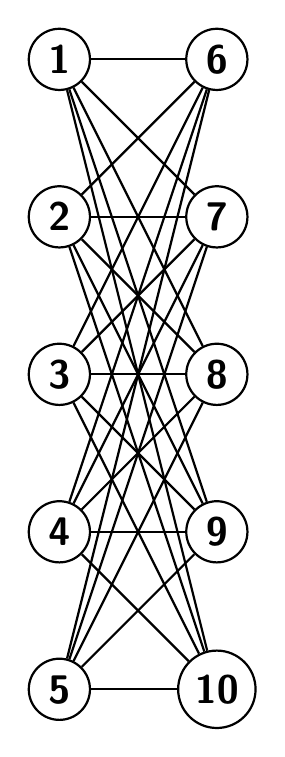
\begin{tikzpicture}[auto, node distance=2cm, thick, every loop/.style={}, main node/.style={circle,draw,font=\sffamily\Large\bfseries}]
  \node[main node] (1) {1};
  \node[main node] (2) [below of=1] {2};
  \node[main node] (3) [below of=2] {3};
  \node[main node] (4) [below of=3] {4};
  \node[main node] (5) [below of=4] {5};
  \node[main node] (6) [right of=1] {6};
  \node[main node] (7) [right of=2] {7};
  \node[main node] (8) [right of=3] {8};
  \node[main node] (9) [right of=4] {9};
  \node[main node] (10) [right of=5] {10};

  \path[every node/.style={font=\sffamily\small}]
    (1) edge node [] {} (6);
  \path[every node/.style={font=\sffamily\small}]
    (2) edge node [] {} (6);
  \path[every node/.style={font=\sffamily\small}]
    (3) edge node [] {} (6);
  \path[every node/.style={font=\sffamily\small}]
    (4) edge node [] {} (6);
  \path[every node/.style={font=\sffamily\small}]
    (5) edge node [] {} (6);
  \path[every node/.style={font=\sffamily\small}]
    (1) edge node [] {} (7);
  \path[every node/.style={font=\sffamily\small}]
    (2) edge node [] {} (7);
  \path[every node/.style={font=\sffamily\small}]
    (3) edge node [] {} (7);
  \path[every node/.style={font=\sffamily\small}]
    (4) edge node [] {} (7);
  \path[every node/.style={font=\sffamily\small}]
    (5) edge node [] {} (7);
  \path[every node/.style={font=\sffamily\small}]
    (1) edge node [] {} (8);
  \path[every node/.style={font=\sffamily\small}]
    (2) edge node [] {} (8);
  \path[every node/.style={font=\sffamily\small}]
    (3) edge node [] {} (8);
  \path[every node/.style={font=\sffamily\small}]
    (4) edge node [] {} (8);
  \path[every node/.style={font=\sffamily\small}]
    (5) edge node [] {} (8);
  \path[every node/.style={font=\sffamily\small}]
    (1) edge node [] {} (9);
  \path[every node/.style={font=\sffamily\small}]
    (2) edge node [] {} (9);
  \path[every node/.style={font=\sffamily\small}]
    (3) edge node [] {} (9);
  \path[every node/.style={font=\sffamily\small}]
    (4) edge node [] {} (9);
  \path[every node/.style={font=\sffamily\small}]
    (5) edge node [] {} (9);
  \path[every node/.style={font=\sffamily\small}]
    (1) edge node [] {} (10);
  \path[every node/.style={font=\sffamily\small}]
    (2) edge node [] {} (10);
  \path[every node/.style={font=\sffamily\small}]
    (3) edge node [] {} (10);
  \path[every node/.style={font=\sffamily\small}]
    (4) edge node [] {} (10);
  \path[every node/.style={font=\sffamily\small}]
    (5) edge node [] {} (10);
\end{tikzpicture}
\end{center}
\newpage
\subsection*{The Degree Sum Formula}
The degree of a vertex is the number of edges in this vertex. Denoted deg(x).
If G is a graph, then the sum of the degrees of the vertices in G is always twice the number of edges in G.

\subsection*{Trees}
A tree is a graph $T$ that is connect and has no cycle graph $C_n$ as a subgraph.

\section*{Proofs}
\subsection*{Direct Proof}
A direct proof is when you take simple known facts, axioms and theorems and 
work them algebraically until you prove the thing you are looking for is true or false.
For statements like 'p implies q' or 'if p then q' we can assume p is true and use 
our known facts/algebra to prove q.
\subsection*{Proof by Contradiction}
Say we have a fact p we want to prove is true. We assume p is false then reach
a contradiction so in fact p \underline{must} be true. Say we want to prove 
p implies q. Then we can assume p is true, but q is false. Then we reach a contradiction.
\subsection*{Proof by Cases}
Say we want to prove a statement in the form 'for all numbers/graphs/etc' but 
the 'numbers/graphs/etc' can be thought of as several families so we deal with each 
separately in different 'cases'. Eg. we could consider odd \& even numbers.
\subsection*{Proof by Construction}
Proof by construction is a bit of an odd ball but can be brought down to simply 
producing an example of what you are trying to prove. If the statement is 
of the form "there exists x" it is a valid proof to just produce a numerical/physical
example otherwise you must work in general i.e "a graph with n vertices".
\subsection*{Proof by Induction}
\end{document}
